% !TeX encoding = UTF-8
% !TeX spellcheck = en_GB
% !TeX root = ../thesis.tex

\chapter{Evaluation and Discussion}
\label{chapter:evaluation}

This chapter presents the evaluation of Threat Detector and its integration with PCAPdroid. The focus of this chapter is to assess the applicability and feasibility of this setup in real-world scenarios. It demonstrates that the existing design effectively captures, analyses, and reports malicious network activities in a user-friendly and practical manner. Moreover, it discusses the observed limitations and provides a performance assessment. Finally, it concludes with some suggestions for further research and improvements.

\section{Assessment Methodology}
The evaluation of Threat Detector as a system was primarily based on a qualitative approach. In this approach the application was tested using a Samsung Galaxy S22 mobile phone with Android 13 (API level 33) installed.

The evaluation is based on the following criteria:
\begin{itemize}
	\item \textbf{Ease of setup and configuration:} how easy and straightforward the setup process was for the users while installing and interacting with Threat Detector and PCAPdroid.
	\item \textbf{Reliability of IP-to-application mapping:} the ability of Threat Detector to correctly associate the network information with the originating applications.
	\item \textbf{Effectiveness of threat identification:} how reliable the threat intelligence is based on the AbuseIPDB lookups.
	\item \textbf{Responsiveness and stability:} how smoothly Threat Detector handled real-time data without considerably slowing the system down.
	\item \textbf{User Experience and interface clarity:} whether users were able to easily interact with Threat Detector and interpret the lookup reports without comprehensive technical expertise.
\end{itemize}

To simulate real-world conditions, Threat Detector went through a series of tests under typical usage patterns such as web-browsing, social media interactions, video streaming, and application usage associated with a remote back-end system. The Android phone remained connected to both mobile data and Wi-Fi during various test sessions to observe its functionality and stability.



\section{Usability Evaluation}

\subsection*{Setup and Integration Experience}
Setting up Threat Detector and PCAPdroid required minimal configuration and adjustments. Users were only needed to select TCP exporter option, make sure of the default values in the collector settings, and finally activate the PCAPdroid extension radio button. This process was earlier demonstrated in the previous chapter as shown in \cref{fig:PCAPdroid Traffic Dump and Exporter Settings}.

The usability of Threat detector was tested by four volunteers familiar with Android and little experience or knowledge about network analysis and the associated tools. All of the participants were able to complete the setup process under 2 minutes.

Participants were asked to report a simplicity score for the setup process and give a number representing the complexity level (5 being the easiest) of the setup process. \cref{fig:usability_ratings} illustrates the aggregated results.

\begin{figure}[H]
	\centering
	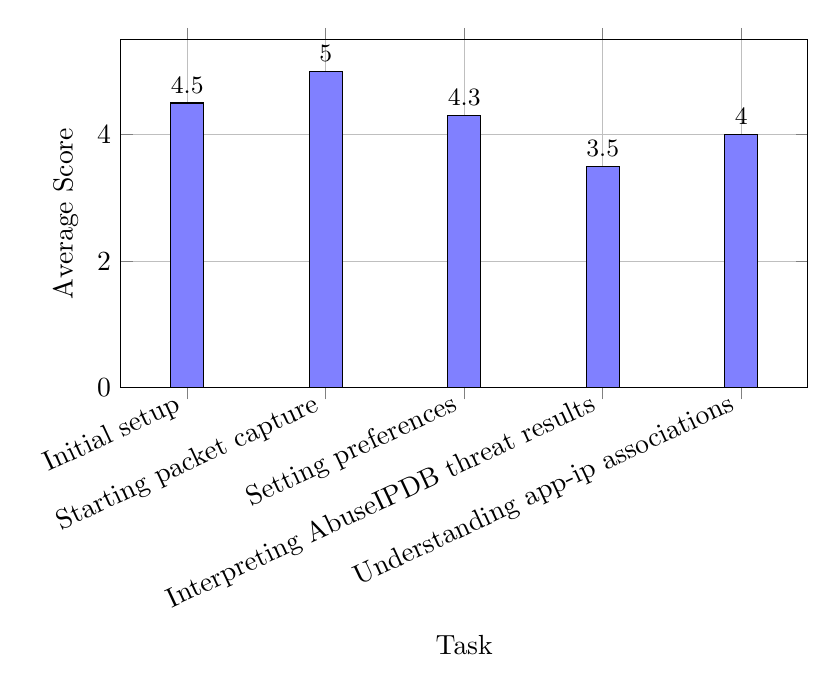
\begin{tikzpicture}
		\begin{axis}[
			ybar,
			bar width=12pt,
			width=0.85\linewidth,
			height=6cm,
			xlabel={Task},
			ylabel={Average Score},
			ymin=0, ymax=5.5,
			symbolic x coords={
				Initial setup,
				Starting packet capture,
				Setting preferences,
				Interpreting AbuseIPDB threat results,
				Understanding app-ip associations
			},
			xtick=data,
			x tick label style={rotate=25, anchor=east},
			nodes near coords,
			nodes near coords align={vertical},
			every node near coord/.append style={font=\small},
			enlarge x limits=0.12,
			grid=major,
			]
			\addplot[fill=blue!50!white] coordinates {
				(Initial setup,4.5)
				(Starting packet capture,5)
				(Setting preferences, 4.3)
				(Interpreting AbuseIPDB threat results,3.5)
				(Understanding app-ip associations,4.0)
			};
		\end{axis}
	\end{tikzpicture}
	\caption{Average simplicity ratings for major tasks, Own Creation}
	\label{fig:usability_ratings}
\end{figure}

In conclusion, all the participants found the process of setting up and the integration taking place between PCAPdroid and Threat Detector to be easy to go through. Furthermore, the process was made easier when the participants understood the cooperation between PCAPdroid and Threat Detector regarding which application is responsible for packet capture and which one is handling the threat intelligence and data depiction.

\subsection*{UI and UX}
The graphical interface of Threat Detector prioritizes simplicity and clarity. It consists of Monitor and Logs pages to display server status and capture traffic metadata accompanied by the threat intelligence information queried from AbuseIPDB. The users gave positive feedback regarding the server status colour coding (green for active and purple for inactive) in addition to light red indicating an IP address with a confidence score above the defined threshold.

However, some participants suggested that the details page shown in \cref{fig:IP_Details_Page} can be cluttered with too much information and can be shown in a more organized manner. Furthermore, in case of excessive usage, the logs list can contain too many items that might be frustrating for users to scroll through to search for a specific application. Therefore, a search functionality was suggested which can be implemented in the future revisions.

\cref{fig:UI_clarity} illustrates the user-reported ease of use for interface clarity. The results shown below are based on the comparison between Threat Detector and other modern application UI, made by the participants.

\begin{figure}[H]
	\centering
	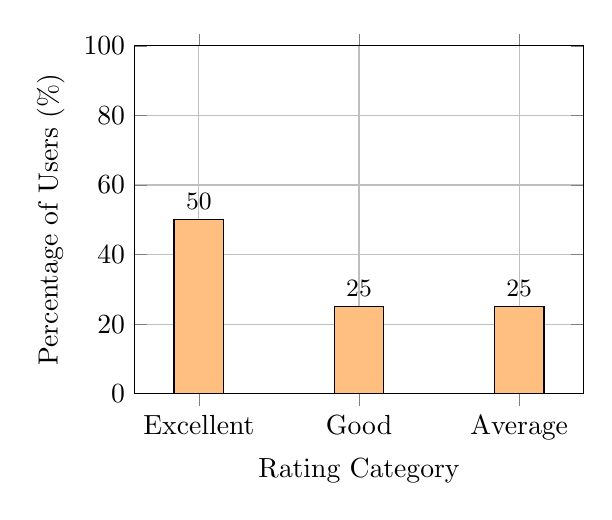
\begin{tikzpicture}
		\begin{axis}[
			ybar,
			bar width=18pt,
			width=0.6\linewidth,
			height=6cm,
			xlabel={Rating Category},
			ylabel={Percentage of Users (\%)},
			ymin=0, ymax=100,
			symbolic x coords={Excellent,Good,Average},
			xtick=data,
			nodes near coords,
			nodes near coords align={vertical},
			every node near coord/.append style={font=\small},
			grid=major,
			enlarge x limits=0.2,
			]
			\addplot[fill=orange!50!white] coordinates {
				(Excellent,50)
				(Good,25)
				(Average,25)
			};
		\end{axis}
	\end{tikzpicture}
	\caption{Perceived clarity of the Threat Detector user interface, Own Creation}
	\label{fig:UI_clarity}
\end{figure}


\section{Functional Evaluation}

\subsection*{IP-to-Application Mapping}
An important aspect of this project is the feature to map the IP addresses of the outbound traffic packets to their originating applications. This was achieved by correlating the extracted packet UID using VpnService API with Android's package manager. 

In the tests that were done to find out the accuracy of IP to application mapping, Threat Detector managed to achieve almost 91\% accuracy as shown in \cref{fig:app_mapping_accuracy}. From 11 applications tested, only one report was incorrect that stems from the intercepted outbound packets from Android built-in services and not the third party applications. These sorts of incorrect associations can occur mainly when background services reuse sockets or when apps share a common UID due to system-level permissions. 

%The tests include browser, Spotify, Telegram, WhatsApp, Instagram, WG-Gesucht, imo, etc.

\begin{figure}[H]
	\centering
	\begin{tikzpicture}
		\pie[
		text=legend,
		sum=auto,
		radius=2.0,
		color={green!50!white, red!50!white}
		]{
			10/Correctly mapped connections,
			1/Mismatched connections
		}
	\end{tikzpicture}
	\caption{Accuracy of IP-to-application mapping during testing, Own Creation}
	\label{fig:app_mapping_accuracy}
\end{figure}


\subsection*{AbuseIPDB Lookup}
Threat Detector's integration with AbuseIPDB has successfully enriched each of the detected outbound IP addresses with a threat reputation score (confidence score from AbuseIPDB query response). 

During a 5-minute browsing session, almost 28 IP addresses were reported, among which 6 were flagged as malicious with a confidence score above 50.

Participants gave positive feedback about flagging the IP addresses and their originating application in the Logs page in real-time which did not negatively interfere with the network activities. Worth to mention that the caching of most reached IP addresses has accelerated the responsiveness and has improved the efficiency of Threat Detector.

\cref{tab:ip_lookup_results} below depicts the IP lookup results.

\begin{table}[H]
	\centering
	\caption{Summary of IP lookup results during evaluation, Own Creation}
	\label{tab:ip_lookup_results}
	\begin{tabular}{lccc}
		\toprule
		\textbf{Category} & \textbf{Count} & \textbf{Percentage (\%)} \\
		\midrule
		Clean IPs & 24 & 85.71 \\
		Malicious IPs & 3 & 10.71 \\
		Timeout & 1 & 3.58 \\
		\midrule
		\textbf{Total} & \textbf{28} & \textbf{100.0} \\
		\bottomrule
	\end{tabular}
\end{table}



\section{System Performance and Resource Utilisation}
Even though for Threat Detector's performance checking no benchmarking tools were employed, Android Studio's Profiler has resulted some informal measurements.

\cref{fig:Android_Studio_Profiler_Results} shows Threat Detector's Performance.

\begin{figure}[H]
	\centering
	\includegraphics[width = 1\textwidth]{Android_Studio_Profiler.png}
	\caption{Android Studio Profiler Results, Own Creation}
	\label{fig:Android_Studio_Profiler_Results}
\end{figure}

\clearpage
 
The screenshot from Android Studio's Profiler illustrates the CPU and memory usage of Threat Detector. The depicted analysis shows the average CPU usage lies around 6 to 10 percent, while having some spikes reaching 15 percent. Moreover, the memory usage analysis shows that while interacting with the app (area shown with vertical blue lines), average memory consumption lies between 55 to 60 MB. These results exhibit the smoothness and efficiency of Threat Detector when it comes to CPU and memory consumption on an Android phone (tests were done on Samsung Galaxy S22 - API 33 and 34).


\section{Future Work}
Although Threat Detector extends the functionality spectrum of previous Android network monitoring systems such as PCAPdroid with the introduction of real-time threat analysis, it has some room for improvement. It still lacks in some areas that can be of utmost importance compared to fully-fledged monitoring and analysis solutions primarily targeting Personal Computers and enterprise networks, such as Wireshark and SIEM (Security Information and Event Management) systems such as \emph{Splunk}\footnote{\url{https://www.splunk.com/}}\cite{Splunk}.

Future development of Threat Detector could focus on the following key areas:

\begin{enumerate}
	\item \textbf{Packet Blocking Functionality:} Incorporation of an optional firewall layer that could enable blocking the connections to a certain IP endpoint when the outbound IP address is flagged as malicious. This could be implemented using the Android's VpnService \texttt{protect()} API to drop the packets or connections if some particular conditions are met.
	
	\item \textbf{Enhanced Performance Benchmarking:} Future assessments of Threat Detector can be done using Android's built-in benchmark library (\texttt{androidx.benchmark}\footnote{\url{https://developer.android.com/jetpack/androidx/releases/benchmark}}\cite{androidx-benchmark}) to measure memory allocation, CPU time and consumption, and also battery usage more accurately. Additionally, some other profiling tools such as \emph{Systrace}\footnote{\url{https://source.android.com/docs/core/tests/debug/systrace}}\cite{android-systrace}, \emph{Perfetto}\footnote{\url{https://perfetto.dev/}}\cite{perfetto}, and \emph{Battery Historian}\footnote{\url{https://developer.android.com/topic/performance/power/battery-historian}}\cite{android-battery-historian} can be used for further measurements.
	
	\item \textbf{Historical Data Visualization:} Implementing a persistent database (e.g. Room) to manage and store more modifiable preferences and keep track of the applications that consistently connect to potentially high-risk IP addresses.
	
	\item \textbf{Automated Testing Frameworks:} Integration with \emph{Espresso}\footnote{\url{https://developer.android.com/training/testing/espresso/}}\cite{android-Espresso} and \emph{JUnit}\footnote{\url{https://developer.android.com/training/testing/local-tests}}\cite{android-Junit} could potentially automate user flows for a more systematic and large-scale testing.
	
	\item \textbf{Improved User Interface with Filters:} Addition of sorting, searching, and filtering capabilities to improve efficiency while monitoring large traffic volumes.
	
	\item \textbf{Privacy and GDPR\footnote{\url{https://gdpr-info.eu/}}\cite{General-Data-Protection-Regulation} Considerations:} Ensuring the anonymization of the IP lookups and further features to comply with data protection standards.
	
	\item \textbf{Integration of Additional Intelligence Sources:} Expanding the threat intelligence sources by incorporating the API from various providers such as \emph{VirusTotal}\footnote{\url{https://blog.virustotal.com/2023/02/monitoring-infrastructure.html}}\cite{Virustotal}, \emph{AlienVault OTX}\footnote{\url{https://otx.alienvault.com/}}\cite{AlienVaultOTX}, and \emph{GreyNoise}\footnote{\url{https://www.greynoise.io/}}\cite{GreyNoise}. This decreases the reliance on a single threat intelligence source.	
\end{enumerate}


\section{Summary}
The evaluation demonstrated in this chapter shows that Threat Detector alongside PCAPdroid provides a lightweight, and practical solution for analysing network traffic and identifying potential malicious connections.

While Threat Detector is neither designed nor intended to be used as a commercially-ready detection system, its eases future research and use in industrial constellations and its design balances performance and applicability. The positive user feedback regarding the reliable IP-to-application mapping and AbuseIPDB response accuracy indicate that the system can effectively raise user awareness of threats and application behaviours. With further improvements and enhancements, Threat Detector can become even a more reliable and valuable research tool for mobile network security.


